\label{sec:mute-couche-securite}

La couche sécurité a pour but de garantir l'authenticité et la confidentialité des messages échangés par les noeuds.
Pour cela, elle implémente un mécanisme de chiffrement de bout en bout.

Pour chiffrer les messages, MUTE utilise un mécanisme de chiffrement à base de clé de groupe.
Le protocole choisi est le protocole Burmester-Desmedt \cite{1995-burmester-desmedt}.
Il nécessite que chaque noeud possède une paire de clés de chiffrement et enregistre sa clé publique auprès d'un PKI\footnote{\acf{PKI} : Infrastructure de gestion de clés}.

Afin d'éviter qu'un \ac{PKI} malicieux n'effectue une attaque de l'homme au milieu sur la collaboration, les noeuds doivent vérifier le bon comportement des PKI de manière non-coordonnée.
À cet effet, MUTE implémente le mécanisme d'audit de PKI Trusternity \cite{2018-trusternity-short, 2018-trusternity-long}.
Son fonctionnement nécessite l'utilisation d'un registre publique sécurisé \emph{append-only}, \ie une blockchain.\\

L'architecture système nécessaire pour la couche sécurité est présentée dans la \autoref{fig:architecture-systeme-trusternity}.

\begin{figure}[!ht]
  \centering
  \includegraphics[page=4, trim=3cm 1cm 4cm 1cm, clip, width=.7\linewidth]{img/mute-figures.pdf}
  \caption{Architecture système pour la couche sécurité de MUTE}
  \label{fig:architecture-systeme-trusternity}
\end{figure}

Cette couche sécurité s'ajoute au mécanisme de chiffrement des messages inhérent à \ac{WebRTC}.
Cela nous offre de nouvelles possibilités : plutôt que de créer un réseau \ac{P2P} par document, nous pouvons désormais mettre en place un réseau \ac{P2P} global.
Les messages étant chiffrés de bout en bout, les noeuds peuvent communiquer en toute sécurité et confidentialité par l'intermédiaire de noeuds tiers, \ie des noeuds extérieurs à la collaboration.\\

Une limite de l'approche actuelle est que la clé de groupe change à chaque évolution des noeuds connectés : à chaque connexion ou déconnexion d'un noeud, une nouvelle clé est recalculée avec les collaborateur-rices présents.
Ce facteur de changement de la clé de chiffrement, nécessaire pour garantir la \emph{backward secrecy} et \emph{forward secrecy} (cf. \autoref{def:backward-secrecy}, page \pageref{def:backward-secrecy} et \autoref{def:forward-secrecy}, page \pageref{def:forward-secrecy}), induit plusieurs problèmes.

Tout d'abord, ce facteur nous empêche de réutiliser cette même clé de chiffrement pour mettre en place un mécanisme de stockage des opérations chiffrées chez un ou des tiers, \eg sur des noeuds du réseau \ac{P2P} extérieurs à la collaboration ou sur des agents de messages.

Le stockage des opérations chiffrées chez des tiers est une fonctionnalité qui améliorerait l'utilisabilité de l'application sans sacrifier la confidentialité des données.
En effet, elle permettrait à un noeud déconnecté de manière temporaire de récupérer à sa reconnexion les modifications effectuées entretemps par ses collaborateur-rices, même si celleux-ci se sont depuis déconnecté-es.

Cependant, la clé de chiffrement est modifiée à la déconnexion du noeud.
Ainsi, les opérations suivantes sont chiffrées avec une nouvelle clé que le noeud déconnecté ne possède pas.
À sa reconnexion, ce dernier ne sera pas en mesure de déchiffrer et d'intégrer les opérations effectuées en son absence.

L'évolution de la clé de chiffrement de groupe à chaque connexion ou déconnexion d'un noeud est donc incompatible avec l'utilisation de cette même clé pour le stockage sécurisé des opérations chez des tiers.
Une autre clé de chiffrement, dédiée, devrait donc être mise en place.\\

Une seconde limite liée à ce facteur d'évolution est la complexité en temps du protocole de génération de la clé de groupe.
En effet, nos évaluations ont montré que ce protocole met jusqu'à 6 secondes pour s'exécuter.

Dans le cadre d'un système \ac{P2P} à large échelle sujet au churn, des périodes d'activités où des noeuds se connectent et déconnectent toutes les 6 secondes sont à envisager.
Lors de tels pics d'activités, les noeuds seraient incapables de collaborer, faute de clé de chiffrement de groupe.
Il convient donc soit d'étudier l'utilisation d'autres protocoles de génération de clés de chiffrement de groupe plus efficaces, soit de considérer relaxer les garanties de \emph{backward secrecy} et de \emph{forward secrecy} dans le cadre des collaborations à large échelle.
